\documentclass[8pt]{beamer}
\usepackage[utf8]{inputenc}
\usepackage{xcolor}
\usepackage{colortbl}
\usepackage{epsfig}
% \usepackage{cancel}
\usepackage{ulem}
% \usepackage{threeparttable} % Joao Pela: 
\usepackage{amsmath}
\usepackage{hyperref}
\usepackage{appendixnumberbeamer}
% \usepackage{feynmp}         % For latex produced Feynman Diagrams

% Rule for feynmp diagrams to be considered graphics
% \DeclareGraphicsRule{*}{mps}{*}{}
% 
% % New compile sequence for feynmp
% \makeatletter
% \def\endfmffile{%
%   \fmfcmd{\p@rcent\space the end.^^J%
%           end.^^J%
%           endinput;}%
%   \if@fmfio
%     \immediate\closeout\@outfmf
%   \fi
%   \ifnum\pdfshellescape=\@ne
%     \immediate\write18{mpost \thefmffile}%
%   \fi}
% \makeatother

\usetheme{Madrid}

\author[J. Pela]{João Pela}
\title[MC VBF QCD]{MC VBF+MET QCD Samples Studies}
\institute[ICL]{Imperial College London}
\date{2014-03-04}

% The log drawn in the upper right corner.
\logo{\includegraphics[height=0.115\paperheight]{img/Logo_CMSICL.png}}

\begin{document}
\setlength{\unitlength}{1mm}

% ###################################################
\begin{frame}
  \titlepage
\end{frame}

% ###################################################
\begin{frame}{Today's presentation}
 
\begin{block}{Topics}
 
\begin{itemize}
  \item Event with fake met study
  \item GenJets Filter with $\Delta\phi$ cut
\end{itemize}
 
\end{block}

\end{frame}

% ###################################################
\begin{frame}{Introduction}

QCD are by far the most frequent processes in collisions at CMS. The elevated cross sections of such processes mean it is normally impossible to generate samples big enough to simulate 
significant amounts of of equivalent luminosity so they can be used in data analysis.

\begin{block}{Methodology}

In order to overcome this problem we generated MC QCD samples with MET plus VBF-like jets.
\begin{itemize}
  \item Real MET (vectorial sum of generator level neutrino $p_T$)
  \item VBF-like jets (AK5 generator level jets)
\end{itemize}

\end{block}

This type of event have a significantly smaller cross section and so to simulate high integrated luminosity samples. 
 
\end{frame}

% ###################################################
\begin{frame}{MC Filter Details}
 
\begin{block}{MC Filter: Vectorial sum of neutrino $E_T$}

  \begin{itemize}
     \item $\sum E_\perp(\vec{\nu}) > 40$ $GeV$
  \end{itemize}

\end{block}

\begin{block}{MC Filter: Dijet Filter}

  \begin{itemize}
    \item Select jets with:
    \begin{itemize}
      \item $p_\perp>20$ $GeV$
      \item $|\eta|<5.0$
    \end{itemize}
    \item From selected jets at least one pair with:
    \begin{itemize}
      \item $m_{jj}>700$ $GeV$
      \item $\Delta\eta>3.2$
    \end{itemize}    
  \end{itemize}

\end{block}

\end{frame}

% ###################################################
\begin{frame}{Fake MET variable dependency I}
 
\begin{block}{How:}

  \begin{itemize}
    \item Next plots are produced with the following conditions:
    \begin{itemize}
      \item Pass VBF trigger (L1+HLT)
      \item Same point of the prompt selection where BDT was trained. Implies passing vetos, having 2 reconstructed jets, etc.
      \item Pass generator jets cut (same as MC VBF QCD samples)
    \end{itemize}
  \end{itemize}

\end{block}

\begin{columns}

\column[t]{0.45\linewidth}
\begin{block}{$MET_{RECO}-MET_{GEN}$ vs $p_T^{jet1}$}
 
\centering
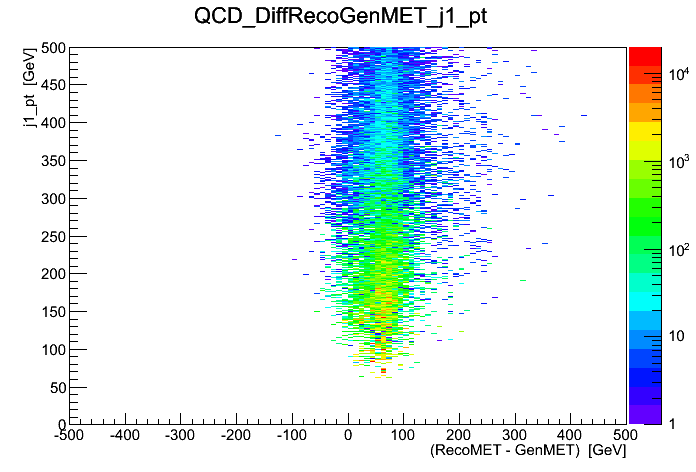
\includegraphics[width=\linewidth]{img/QCD_DiffRecoGenMET_j1_pt.png} 

\end{block}

\column[t]{0.45\linewidth}
\begin{block}{$MET_{RECO}-MET_{GEN}$ vs $p_T^{jet2}$}
 
\centering
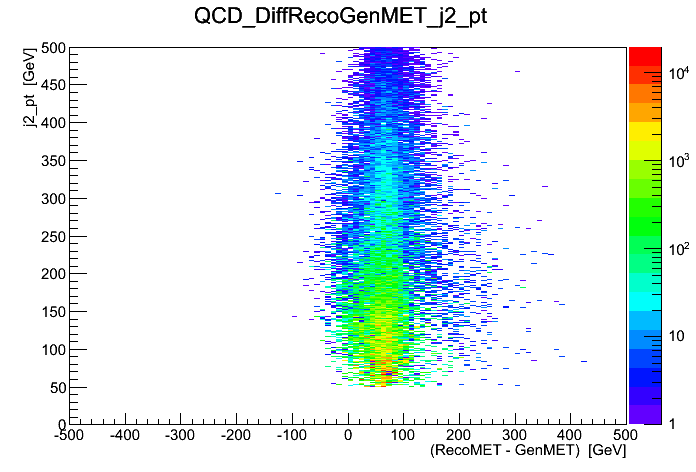
\includegraphics[width=\linewidth]{img/QCD_DiffRecoGenMET_j2_pt.png} 
 
\end{block}

\end{columns}

$p_T$ of the jets seams to be fairly decorated with the difference between RECO and GEN MET 

\end{frame}

% ###################################################
\begin{frame}{Fake MET variable dependency II}
 
\begin{columns}

\column[t]{0.45\linewidth}
\begin{block}{$MET_{RECO}-MET_{GEN}$ vs $HT$}

\centering
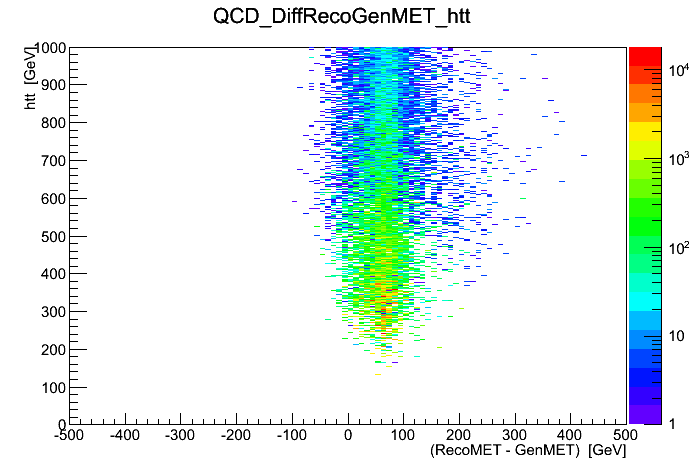
\includegraphics[width=\linewidth]{img/QCD_DiffRecoGenMET_htt.png} 
 
\end{block}

\column[t]{0.45\linewidth}
\begin{block}{$MET_{RECO}-MET_{GEN}$ vs $\sum p_T(j_1,j_2,MET)$}

\centering
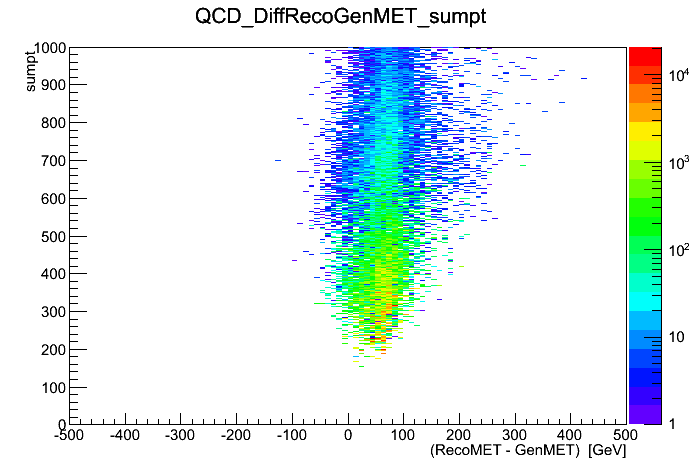
\includegraphics[width=\linewidth]{img/QCD_DiffRecoGenMET_sumpt.png} 
 
\end{block}

\end{columns}

Energy sums also look fairly decorated with the difference between RECO and GEN MET. But as expected the more energy
is available the bigger is the tail into higher energy of fake met.

\end{frame}

% ###################################################
\begin{frame}{Fake MET variable dependency III}
 
\begin{columns}

\column[t]{0.45\linewidth}
\begin{block}{$MET_{RECO}-MET_{GEN}$ vs $MET_{RECO}$}

\centering
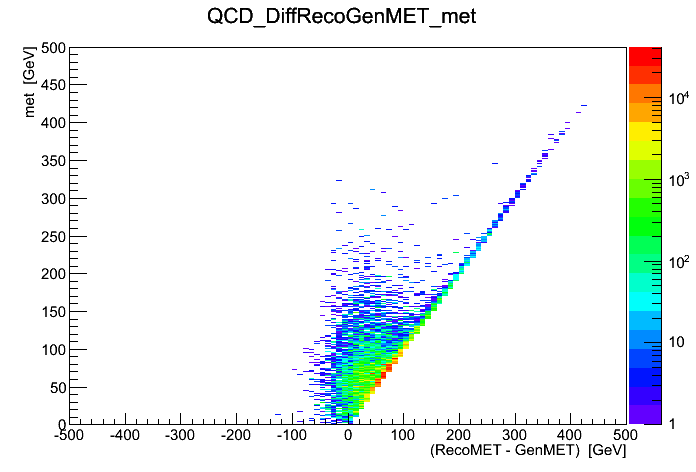
\includegraphics[width=\linewidth]{img/QCD_DiffRecoGenMET_met.png} 
 
\end{block}

\column[t]{0.45\linewidth}
\begin{block}{$MET_{RECO}-MET_{GEN}$ vs $MET_{Sig}$}

\centering
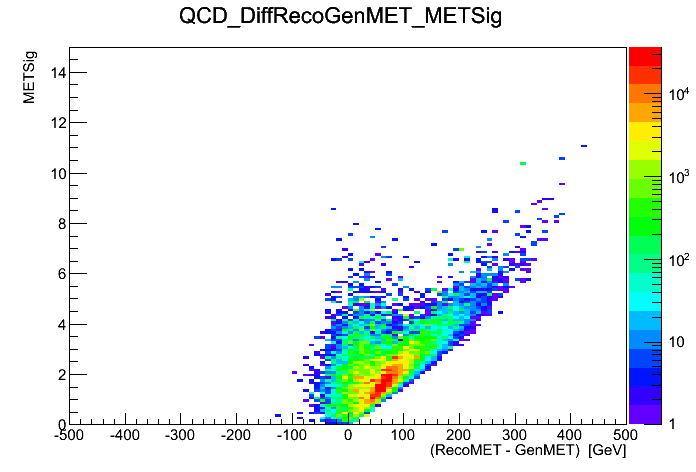
\includegraphics[width=\linewidth]{img/QCD_DiffRecoGenMET_METSig.png} 
 
\end{block}

\end{columns}

\begin{itemize}
  \item Left Plot: We can see clearly the 2 populations of events. Note that most events are fake met.
  \item Right Plot: MET significance is NOT helpful to discriminate against fake met. Events with high fake met also have high met significance... 
\end{itemize}

\end{frame}

% ###################################################
\begin{frame}{Fake MET variable dependency IV}
 
\begin{columns}

\column[t]{0.45\linewidth}
\begin{block}{$MET_{RECO}-MET_{GEN}$ vs $\Delta\phi_{jet-jet}$}
 
\centering
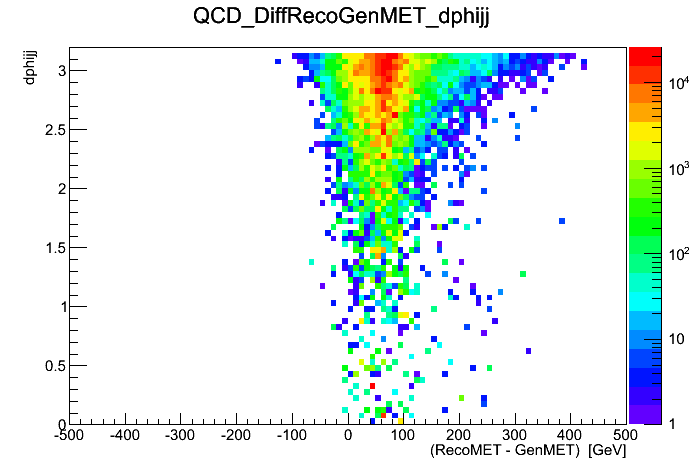
\includegraphics[width=\linewidth]{img/QCD_DiffRecoGenMET_dphijj.png} 
 
\end{block}

\column[t]{0.45\linewidth}
\begin{block}{$MET_{RECO}-MET_{GEN}$ vs $BDT_{Score}$}

\centering
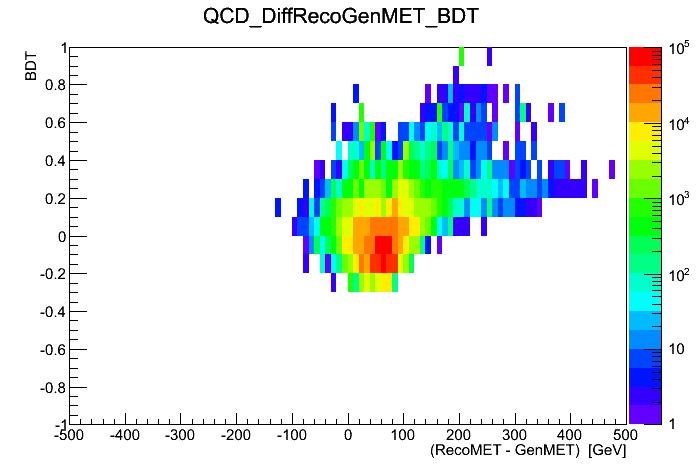
\includegraphics[width=\linewidth]{img/QCD_DiffRecoGenMET_BDT.png} 
 
\end{block}

\end{columns}

\begin{itemize}
  \item Left Plot: We can see that most population of fake met events have high $\Delta\phi_{jet-jet}$ as expected but significant tails can be seen still at low values
  \item Right Plot: Here we can see that the BDT is not being very efficient in rejecting fake met events.
\end{itemize}

\end{frame}

% ###################################################
\begin{frame}{Fake MET variable dependency V}
 
\begin{columns}

\column[t]{0.45\linewidth}
\begin{block}{$MET_{RECO}-MET_{GEN}$ vs $\Delta\phi_{jet_1-MET}$}
 
\centering
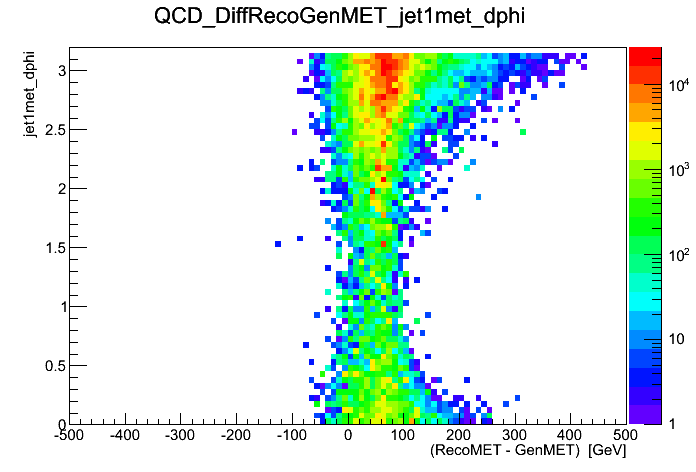
\includegraphics[width=\linewidth]{img/QCD_DiffRecoGenMET_jet1met_dphi.png} 
 
\end{block}

\column[t]{0.45\linewidth}
\begin{block}{$MET_{RECO}-MET_{GEN}$ vs $\Delta\phi_{jet_2-MET}$}

\centering
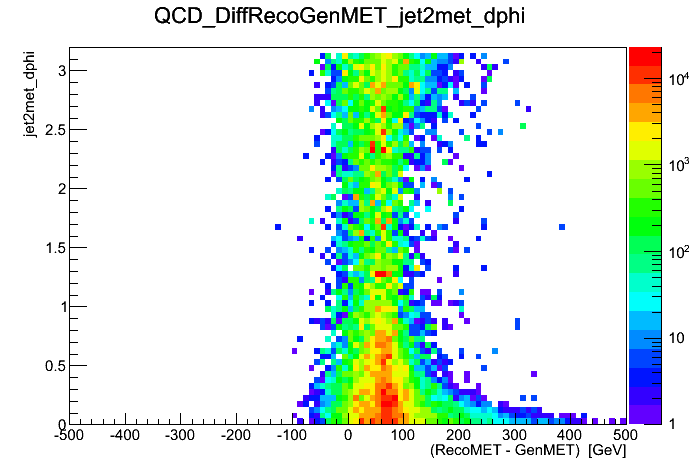
\includegraphics[width=\linewidth]{img/QCD_DiffRecoGenMET_jet2met_dphi.png} 
 
\end{block}

\end{columns}

We can see here strong correlations between fake met and angles between met and jets.

\begin{itemize}
  \item Left Plot: Most events with high fake met are in the pi or zero angles to leading jet 
  \item Right Plot: Similar but reversed, most events with fake met are in 0 or pi angles to leading jets
\end{itemize}

Implies that a major cause of fake met miss measurement sub-leading and leading jets. We can try to select events based on this variables.

\end{frame}

% ###################################################
\begin{frame}{Selecting based on jet(1,2) $\Delta\phi$ to met I}
 
We will select events based on jet(1,2) $\Delta\phi$ to met
\begin{itemize}
  \item WP1: jet1 to met $0.5<\Delta\phi<2.5$
  \item WP2: jet2 to met $0.5<\Delta\phi<2.5$
  \item WP3: both conditions 
\end{itemize}

\begin{columns}

\column[t]{0.45\linewidth}
\begin{block}{No cut}
 
\centering
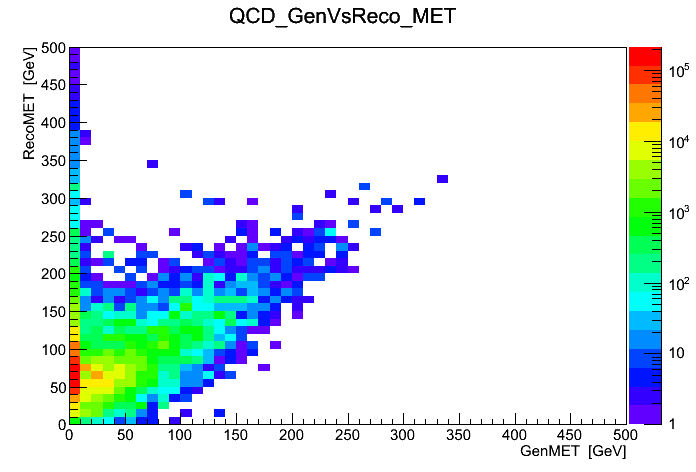
\includegraphics[width=\linewidth]{img/QCD_GenVsReco_MET.png} 
 
\end{block}

\column[t]{0.45\linewidth}
\begin{block}{WP1}

\centering
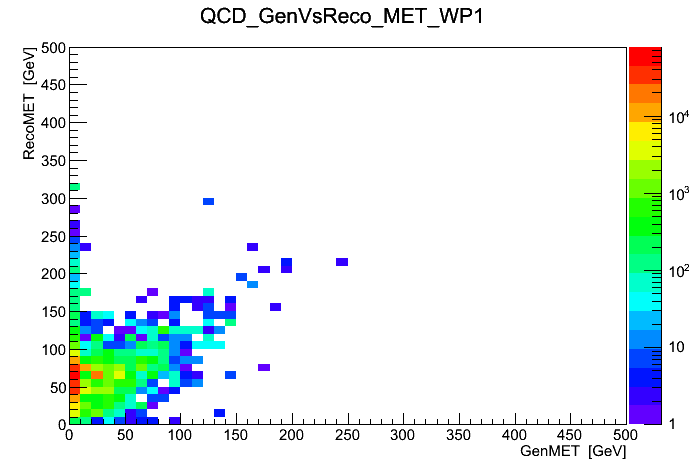
\includegraphics[width=\linewidth]{img/QCD_GenVsReco_MET_WP1.png} 
 
\end{block}

\end{columns}

\end{frame}

% ###################################################
\begin{frame}{Selecting based on jet(1,2) $\Delta\phi$ to met II}
 
\begin{columns}

\column[t]{0.45\linewidth}
\begin{block}{WP2}
 
\centering
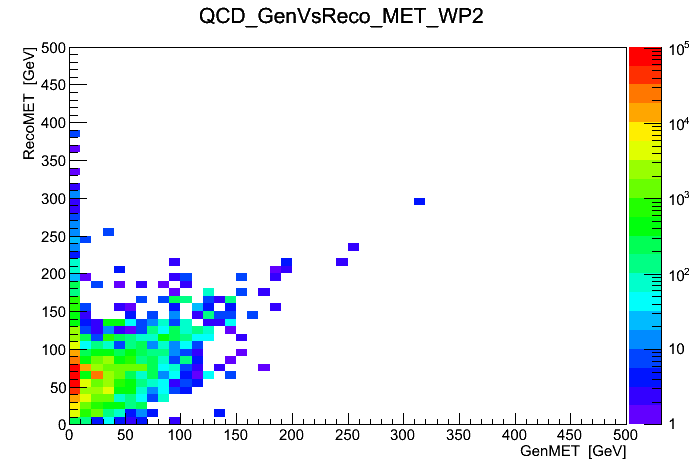
\includegraphics[width=\linewidth]{img/QCD_GenVsReco_MET_WP2.png} 
 
\end{block}

\column[t]{0.45\linewidth}
\begin{block}{WP3}

\centering
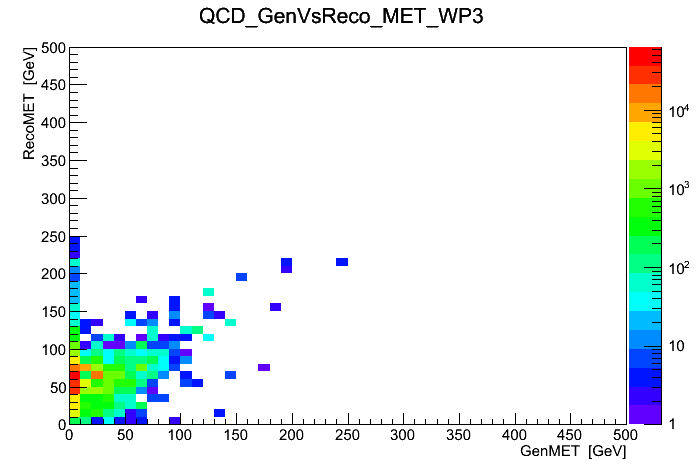
\includegraphics[width=\linewidth]{img/QCD_GenVsReco_MET_WP3.png} 
 
\end{block}

\end{columns}

Cutting on this variables helps to control the fake met tail to high energies.

\end{frame}

% ###################################################
\begin{frame}{Study on GenJet Filter only}

On possibility to avoid the a pre-selection altogether would be to produce new samples with just GenJets filter
but adding more cuts there in other to get additional suppression thus removing the need for a GenMET cut.

The obvious variable to add would be $\Delta\phi$. Have have made a quick study to check this possibility.
 
\begin{block}{1/Efficiency}
 
\resizebox{\linewidth}{!}{
\begin{tabular}{|c|r|r|r|r|r|r|}
\hline
$p_T$ hat                       &  50to80 & 80to120 & 120to170 & 170to300 & 300to470 & 470to600 \\
\hline\hline
Current GenFilters              &  333333 &   24390 &     3413 &      988 &      385 &      239 \\ 
\hline\hline
GenJet Filter $+\Delta\phi<1.5$ &     158 &      78 &       36 &       24 &       14 &       11 \\
GenJet Filter $+\Delta\phi<1.0$ &     204 &     113 &       54 &       33 &       20 &       16 \\ 
\hline
\end{tabular}
}

\end{block}
 
Event using cut as high as $\Delta\phi<1.0$ we are not even close to the necessary event suppression used 
to create the current VBF QCD sample.
  
\end{frame}

% ###################################################
% \begin{frame}{Summary and next steps}
%  
% \begin{block}{Summary:}
%  
% \begin{itemize}
%   \item 
% \end{itemize}
% 
% \end{block}
% 
% \begin{block}{Next Steps:}
%  
% \begin{itemize}
%  \item 
% \end{itemize}
%  
% \end{block}
% 
% \end{frame}


% ###################################################
\appendix
% ###################################################
\begin{frame}
 
\begin{block}

\begin{center}Backup Slides\end{center}

\end{block}

\end{frame}

% % ###################################################
% \begin{frame}{}
% 
% \begin{columns}
% 
% \column[t]{0.35\linewidth}
% \begin{block}{QCD\_Pt-30to50}
%  
% \centering
% % 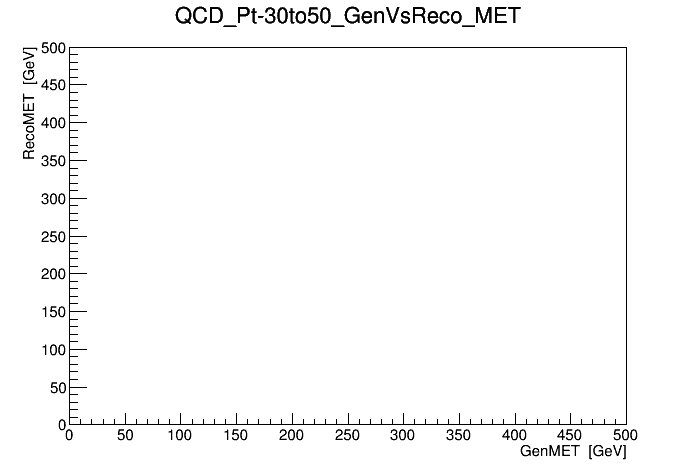
\includegraphics[width=\linewidth]{img/QCD_Pt-30to50_GenVsReco_MET.png} 
%  
% \end{block}
% 
% \begin{block}{QCD\_Pt-80to120}
%  
% \centering
% % 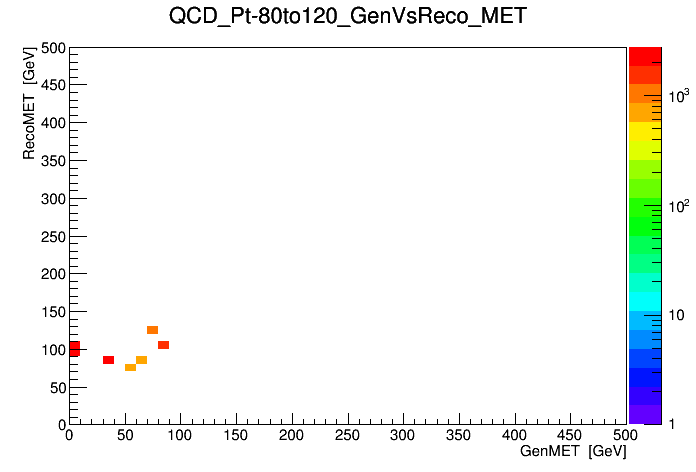
\includegraphics[width=\linewidth]{img/QCD_Pt-80to120_GenVsReco_MET.png} 
%  
% \end{block}
% 
% 
% \column[t]{0.35\linewidth}
% \begin{block}{QCD\_Pt-50to80}
%  
% \centering
% % 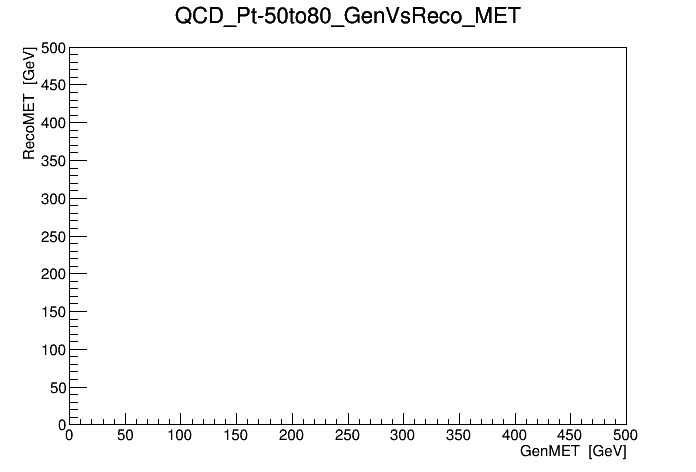
\includegraphics[width=\linewidth]{img/QCD_Pt-50to80_GenVsReco_MET.png} 
%  
% \end{block}
% 
% \begin{block}{QCD\_Pt-120to170}
%  
% \centering
% % 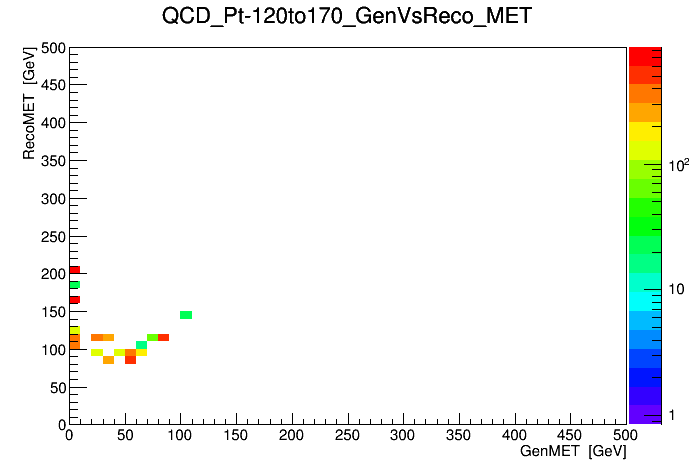
\includegraphics[width=\linewidth]{img/QCD_Pt-120to170_GenVsReco_MET.png} 
%  
% \end{block}
% 
% 
% \end{columns} 
%  
% \end{frame}

\end{document}